\documentclass{beamer}
\mode<presentation> {
%\usetheme{Madrid}
%\usetheme{default}
\usepackage{color}
\definecolor{bottomcolour}{rgb}{0.21,0.11,0.21}
\definecolor{middlecolour}{rgb}{0.21,0.11,0.21}
\setbeamercolor{structure}{fg=white}
\setbeamertemplate{frametitle}[default]%[center]
\setbeamercolor{normal text}{bg=black, fg=white}
\setbeamertemplate{background canvas}[vertical shading]
[bottom=bottomcolour, middle=middlecolour, top=black]
\setbeamertemplate{items}[circle]
\setbeamertemplate{navigation symbols}{} %no nav symbols
\setbeamercolor{block title}{use=structure,fg=white,bg=structure.fg!50!red!50!blue!100!green}
\setbeamercolor{block body}{parent=normal text,use=block title,bg=block title.bg!5!white!10!bg,fg=white}
\setbeamertemplate{navigation symbols}{}
}

\usepackage{graphicx} 
\usepackage{booktabs} 
\usepackage[utf8]{inputenc}  
\usepackage[T1]{fontenc}  
\usepackage{geometry}     
\usepackage[francais]{babel} 
\usepackage{eurosym}
\usepackage{verbatim}
\usepackage{ragged2e}
\justifying

%%%%%%%%%%%%%%%%%%%%%%%%%%%%%%%%%%%%%%%%%%%%%%%%%%%%%%%%%%%%%%%%
%% ccBeamer 0.1, 2007-07-02                                   %%
%% Written by Sebastian Pipping <webmaster@hartwork.org>      %%
%% ---------------------------------------------------------- %%
%% Licensed under Creative Commons Attribution-ShareAlike 3.0 %%
%% http://creativecommons.org/licenses/by-sa/3.0/             %%
%%%%%%%%%%%%%%%%%%%%%%%%%%%%%%%%%%%%%%%%%%%%%%%%%%%%%%%%%%%%%%%%


%% Images
\newcommand{\CcImageBy}[1]{%
	
\includegraphics[scale=#1]{creative_commons/cc_by_30.pdf}%
}
\newcommand{\CcImageCc}[1]{%
	
\includegraphics[scale=#1]{creative_commons/cc_cc_30.pdf}%
}
\newcommand{\CcImageDevNations}[1]{%
	
\includegraphics[scale=#1]{creative_commons/cc_dev_nations_30.pdf}%
}
\newcommand{\CcImageNc}[1]{%
	
\includegraphics[scale=#1]{creative_commons/cc_nc_30.pdf}%
}
\newcommand{\CcImageNd}[1]{%
	
\includegraphics[scale=#1]{creative_commons/cc_nd_30.pdf}%
}
\newcommand{\CcImagePd}[1]{%
	
\includegraphics[scale=#1]{creative_commons/cc_pd_30.pdf}%
}
\newcommand{\CcImageSa}[1]{%
	
\includegraphics[scale=#1]{creative_commons/cc_sa_30.pdf}%
}
\newcommand{\CcImageSampling}[1]{%
	
\includegraphics[scale=#1]{creative_commons/cc_sampling_30.pdf}%
}
\newcommand{\CcImageSamplingPlus}[1]{%
	
\includegraphics[scale=#1]{creative_commons/cc_sampling_plus_30.pdf}%
}


%% Groups
\newcommand{\CcGroupBy}[1]{% zoom
	\CcImageBy{#1}%
}
\newcommand{\CcGroupByNc}[2]{% zoom, gap
	\CcImageBy{#1}\hspace*{#2}\CcImageNc{#1}%
}
\newcommand{\CcGroupByNcNd}[2]{% zoom, gap
	\CcImageBy{#1}\hspace*{#2}\CcImageNc{#1}\hspace*{#2}\CcImageNd{#1}%
}
\newcommand{\CcGroupByNcSa}[2]{% zoom, gap
	\CcImageBy{#1}\hspace*{#2}\CcImageNc{#1}\hspace*{#2}\CcImageSa{#1}%
}
\newcommand{\CcGroupByNd}[2]{% zoom, gap
	\CcImageBy{#1}\hspace*{#2}\CcImageNd{#1}%
}
\newcommand{\CcGroupBySa}[2]{% zoom, gap
	\CcImageBy{#1}\hspace*{#2}\CcImageSa{#1}%
}
\newcommand{\CcGroupDevNations}[1]{% zoom
	\CcImageDevNations{#1}%
}
\newcommand{\CcGroupNcSampling}[2]{% zoom, gap
	\CcImageNc{#1}\hspace*{#2}\CcImageSampling{#1}%
}
\newcommand{\CcGroupPd}[1]{% zoom
	\CcImagePd{#1}%
}
\newcommand{\CcGroupSampling}[1]{% zoom
	\CcImageSampling{#1}%
}
\newcommand{\CcGroupSamplingPlus}[1]{% zoom
	\CcImageSamplingPlus{#1}%
}


%% Text
\newcommand{\CcLongnameBy}{Attribution}
\newcommand{\CcLongnameByNc}{Attribution-NonCommercial}
\newcommand{\CcLongnameByNcNd}{Attribution-NoDerivs}
\newcommand{\CcLongnameByNcSa}{Attribution-NonCommercial-ShareAlike}
\newcommand{\CcLongnameByNd}{Attribution-NoDerivs}
\newcommand{\CcLongnameBySa}{Attribution-ShareAlike}

\newcommand{\CcNote}[1]{% longname
	This work is licensed under the \textit{Creative Commons #1 3.0 License}.%
}


\title[Le chiffrement]{
Ubuntu Party \\
Le chiffrement - introduction} 
\author{Genma}

\begin{document}

%% Titlepage
\begin{frame}
	\titlepage
	\vfill
	\begin{center}
		\CcGroupByNcSa{0.83}{0.95ex}\\[2.5ex]
		{\tiny\CcNote{\CcLongnameByNcSa}}
		\vspace*{-2.5ex}
	\end{center}
\end{frame}


%\begin{frame}
%\frametitle{Plan} 
%\tableofcontents
%\end{frame}

%----------------------------------------------------------------------------------------
%	PRESENTATION SLIDES
%----------------------------------------------------------------------------------------


\begin{frame}
\frametitle{
\includegraphics[scale=0.4]{./Illustrations/Genma.jpg} \ \ \  A propos de moi  }
\begin{columns}[c] 

\column{.55\textwidth} 
\textbf{Où me trouver sur Internet?}
\begin{itemize}
\item Le Blog de Genma : http://genma.free.fr
\item Twitter : http://twitter.com/genma
\end{itemize}

\textbf{Mes centres d'intérêts?}
\\ Plein de choses dont:
\begin{itemize}
\item La veille technologique
\item Le chiffrement
\end{itemize}

\textbf{Ubuntu?}
Depuis la version 4.10...

\column{.5\textwidth} 
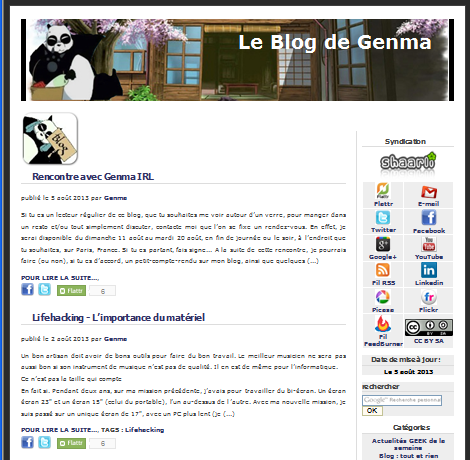
\includegraphics[width=5cm,height=5cm]{./Illustrations/blog.png} 

\end{columns}
\end{frame}


%------------------------------------------------

\begin{frame}
\frametitle{But de cette présentation}

\begin{block}{Ce que cette présentation est}
Cette présentation est une introduction au chiffrement, à son rôle...
\\$\Rightarrow$ Son but est de lancer un débat sur le sujet.
\end{block}

\begin{block}{Ce que cette présentation n'est pas}
Un tutoriel sur le chiffrement de ses e-mails, de son disque dur, des ses communications.
\\$\Rightarrow$  Il y aura des ateliers pour ça.
\end{block}
\end{frame}

%----------------------------------------------------------------------------------------
\begin{frame}
\Huge{\centerline{Le chiffrement, c'est quoi?}}

\begin{center}
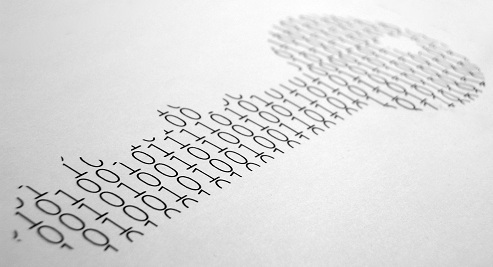
\includegraphics[scale=0.4] {./Illustrations/cryptography.jpg} 
\end{center}
\end{frame}

%------------------------------------------------
\begin{frame}
\frametitle{Définitions - cryptage, crypter, chiffrement ?}

\begin{block}{Le chiffrement}
\justifying{
Le chiffrement consiste à chiffrer un document/un fichier à l’aide d’une clef de chiffrement. 
L’opération inverse étant le déchiffrement. 
}
\end{block}
\begin{block}{Le cryptage}
\justifying{
Le terme « cryptage » est un anglicisme, tiré de l’anglais encryption. 
Le décryptage existe : il s’agit de "casser" un document chiffré lorsqu’on n’en a pas la clef.
}
\end{block}
\begin{block}{La cryptographie}
\justifying{
La science quant-à elle s’appelle  la "cryptographie".
}
\end{block}
\end{frame}

%------------------------------------------------
\begin{frame}
\frametitle{Le chiffrement, comment ça se passe?}

\begin{block}{Le chiffrement symétrique}
\justifying{
Cela consiste à chiffrer un message avec la même clef que celle qui sera utilisé pour le déchiffrement. 
\\
Exemple : le code de César avec un décalage de lettres. A->C, B->D etc.
\\
Nous venons en paix ->  Pqwu xgpqpu gp rckz
\\
On applique le processus inverse pour avoir le message.
}
\end{block}

\begin{block}{Une clef de chiffrement c'est quoi?}
\justifying{

Une clef s'appelle une clef car elle ouvre/ferme le cadenas qu'est l'algorithme de chiffrement utilisé.
\begin{itemize}
\item Ici, l'algorithme est dans la notion de décalage.
\item La clef est le nombre de lettre décallées (ici deux lettres).
\end{itemize}
}
\end{block}

\end{frame}

%------------------------------------------------
\begin{frame}
\frametitle{Le chiffrement asymétrique 1/2}

\begin{block}{Clef publique - clef privée}
\justifying{

Le chiffrement asymétrique repose sur le couple clef publique - clef privée.
\\$\Rightarrow$  Ce qu'il faut comprendre/retenir : 
\begin{itemize}
\item Ma clef privée est secrète.
\item Ma clef publique est distribuée à tous.
\end{itemize}
}
\end{block}

\begin{block}{L'algorithme de chiffrement}
\justifying{
L'algorithme de chiffrement est bien plus complexe que le fait de décaler des lettres ; il repose sur des notions mathématiques (nombre premiers...)
}
\end{block}

\end{frame}

\begin{frame}
\frametitle{Le chiffrement asymétrique 2/2}

\begin{block}{Le chiffrement}
Avec la clef publique de mon correspondant, je chiffre  un fichier.
\\$\Rightarrow$ Le fichier ne peut plus être déchiffré que par la personne qui possède la clef privée correspondant à la clef publique que j'ai utilisée (donc mon correspondant).
\end{block}

\begin{block}{Le déchiffrement}
Avec sa clef privée,  mon correspondant déchiffre le fichier.
\\
$\Rightarrow$ Il peut alors lire le message.
\end{block}

\begin{block}{Cas concret}
Le chiffrement de ses mails avec PGP.
\end{block}
\end{frame}

%----------------------------------------------------------------------------------------
\begin{frame}
\frametitle{PGP, GPG?}
\begin{block}{PGP}
\justifying{
Pretty Good Privacy - PGP est un logiciel de chiffrement et de déchiffrement cryptographique, créé par l'américain Phil Zimmermann en 1991.
}
\end{block}
\begin{block}{OpenPGP}
\justifying{
Ce standard décrit le format des messages, signatures ou certificats que peuvent s'envoyer des logiciels comme GNU Privacy Guard. Ce n'est donc pas un logiciel, mais un format pour l'échange sécurisé de données, qui doit son nom au programme historique Pretty Good Privacy (PGP).
}
\end{block}
\begin{block}{GnuPG}
\justifying{GnuPG (ou GPG, de l'anglais GNU Privacy Guard) est l'implémentation GNU du standard OpenPGP.}
\end{block}
\end{frame}


%----------------------------------------------------------------------------------------
\begin{frame}
\frametitle{Bob envoit un message à Alice}
\begin{center}
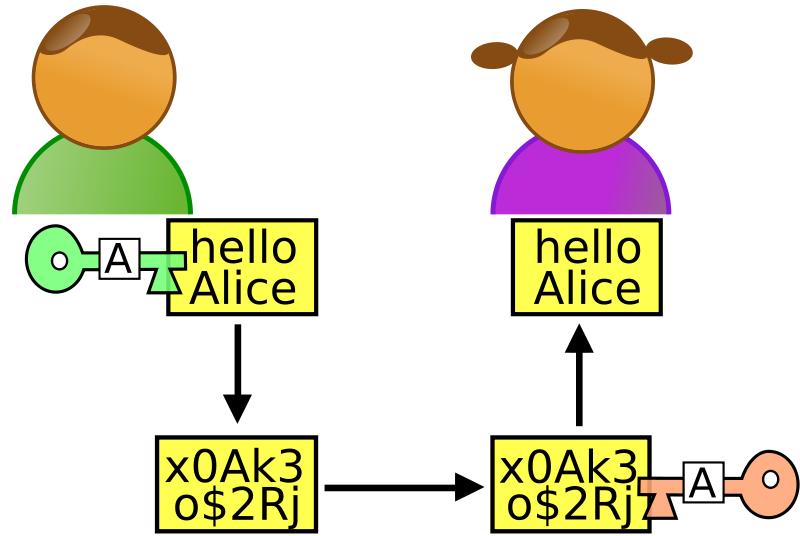
\includegraphics[scale=0.4] {./Illustrations/Alice_et_bob.png} 
\end{center}
\end{frame}


%----------------------------------------------------------------------------------------
\begin{frame}
\Huge{\centerline{Pourquoi chiffrer?}}
\begin{center}
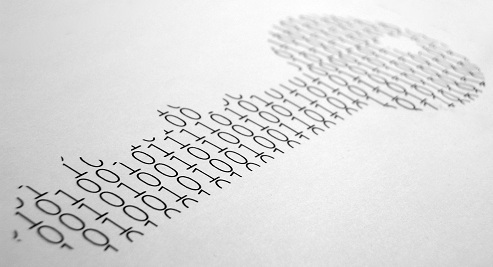
\includegraphics[scale=0.4] {./Illustrations/cryptography.jpg} 
\end{center}
\end{frame}

%------------------------------------------------
\begin{frame}
\frametitle{Chiffrer - Les arguments contre}

\justifying{
\begin{block}{Personne ne le fait...}
FAUX. Sans le savoir, vous le faîtes tous les jours.
\\
Exemple 1: "le cadenas" quand on se connecte
\\  Exemple 2: La clef du Wifi.
\end{block}

\begin{block}{Je n'ai rien à cacher...}
FAUX. Qui accepterait que le facteur lise son courrier médical ?
\end{block}

\begin{block}{Le chiffrement, c'est pour les pédonazis de l'Internet...}
FAUX. Cas des journalistes/blogueurs dissidents qui dénoncent des dictatures...
\end{block}
}
\end{frame}

%------------------------------------------------
\begin{frame}
\frametitle{Chiffrer - Les arguments pour}

\begin{block}{Le chiffrement, ce n'est pas si compliqué}
Ce n'est pas plus compliqué que d'utiliser un "logiciel" ; i faut comprendre le principe et c'est du clickodrome.
\end{block}

\begin{block}{Protection et sécurité}
Mes données personnelles, sensibles sont protégées. Cf. PRISM, NSA...
\end{block}

\begin{block}{Confidentialité}
Seule la personne à qui est destiné le "message" est en mesure de le lire.
\end{block}

\end{frame}

%------------------------------------------------
\begin{frame}
\frametitle{Limites du chiffrement}
\begin{block}{Ce qui est chiffré aujourd'hui pourra être déchiffré demain}
\justifying{
Les ordinateurs de demain pourront permettre de décrypter les données chiffrées aujourd'hui.
}
\end{block}

\begin{block}{Si on perd la clef}
On n'a plus accès aux données.
\end{block}

\begin{block}{Métadonnées, graphe social}
\justifying{
\textbf{PGP ne protège pas contre l'analyse des métadonnée (serveurs de transit, adresses, headers, sujet).}
Ne pas oublier de nettoyer les métas-données des fichiers (tag EXIF des photos, documents de bureautiques avec le suivi des modifications).
DNS, cas du tracking Internet...
}
\end{block}

\end{frame}

%----------------------------------------------------------------------------------------
\begin{frame}
\frametitle{Le chiffrement et la loi}
\justifying{
En France, la loi considère donc que l’utilisation de moyens de cryptologie est libre (LCEN article 30-1) et il n'y a donc, actuellement pas de limite à la taille de la clef de chiffrement que l'on peut utiliser.
\\~\\
En cas de perquisition,le refus de remise de la clef de chiffrement peut entraîner 3 ans d’emprisonnement ainsi que 45000\euro{} d’amende.
\\~\\
Cette peine est aggravée dans le cas où le chiffrement a été utilisé pour commettre un délit. 
\\~\\
Il est donc recommandé de donner la clef de déchiffrement, sauf dans le cas où les données déchiffrées entrainerait une procédure judiciaire dont la peine finale serait supérieure à celle de l'entrave à l'enquête judiciaire.
}
\end{frame}


%----------------------------------------------------------------------------------------
\begin{frame}
\Huge{\centerline{Quoi et comment chiffrer?}}
\begin{center}
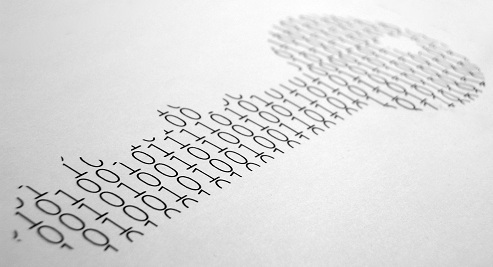
\includegraphics[scale=0.4] {./Illustrations/cryptography.jpg} 
\end{center}
\end{frame}

%------------------------------------------------
\begin{frame}
\frametitle{Quoi et comment chiffrer?}
\justifying{
\begin{block}{En local - ses données}
\begin{itemize}
\item Son disque dur
\item Sa clef USB
\item Son smartphone
\end{itemize}
\end{block}

\begin{block}{En réseau - ses communications}
\begin{itemize}
\item Https : utilisation de l'extension HTTPSEveryWhere pour Firefox  
\item Ses e-mails : utilisation de GPG via Enigmail pour Thunderbird
\item Sa connexion : utiliser un VPN, SSH, la clef "WIFI".
\end{itemize}
\end{block}

\begin{block}{}
$\Rightarrow$ \`A chaque "usage", il y a une solution de chiffrement possible.
\end{block}
}
\end{frame}

%----------------------------------------------------------------------------------------
\begin{frame}
\frametitle{Mise en pratique aujourd'hui et demain}

\begin{block}{Clefs PGP et chiffrement des mails}
\justifying{

\begin{columns}[c] 
\column{.7\textwidth} 
\begin{itemize}
\item Création et gestion de ses clefs avec Seahorse
\item Utilisation d'Enigmail et Thunderbird
\item Signature des clefs
\end{itemize}

\column{.3\textwidth} 
 
\includegraphics[scale=0.4] {./Illustrations/seahorse.jpg} 
 
\includegraphics[scale=0.2] {./Illustrations/thunderbird.png} 
\end{columns}
}
\end{block}

\begin{block}{TrueCrypt, chiffrement des disques durs et clefs USB}
\justifying{
\begin{columns}[c] 
\column{.7\textwidth} 
\begin{itemize}
\item Installation de TrueCrypt
\item Création de volume TrueCrypt
\end{itemize}
\column{.3\textwidth} 
 
\includegraphics[scale=0.2] {./Illustrations/truecrypt.png} 
\end{columns}
}
\end{block}

\begin{block}{Tor}
\justifying{
\begin{columns}[c] 
\column{.7\textwidth} 
\begin{itemize}
\item TorBrowser Bundle
\item TAILS : Live cd-debian avec Tor
\end{itemize}
\column{.3\textwidth} 
 
\includegraphics[scale=0.2] {./Illustrations/tor.png} 
\end{columns}
}
\end{block}

\end{frame}

%----------------------------------------------------------------------------------------
\begin{frame}
\Huge{\centerline{Vous êtes attendus - les bienvenus}}
\Huge{\centerline{pour discuter, tester, essayer...}}
\begin{center}

\includegraphics[scale=0.4] {./Illustrations/cryptoparty.jpg} 
\end{center}
\end{frame}

%----------------------------------------------------------------------------------------
\begin{frame}
\Huge{\centerline{Conclusion}}
\begin{center}
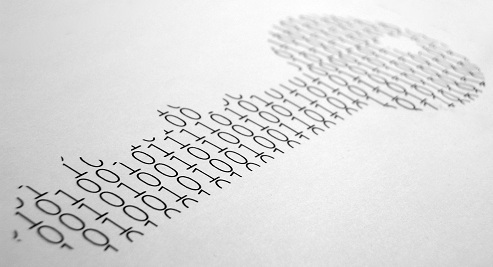
\includegraphics[scale=0.4] {./Illustrations/cryptography.jpg} 
\end{center}
\end{frame}


%----------------------------------------------------------------------------------------
\begin{frame}
\frametitle{Conclusion}
\justifying{
Chiffrer est légal et n'est pas réservé aux paranoïaques.
\\~\\
Chiffrer devient une nécessite dans un monde où les communications sont surveillées.
\\~\\
Chiffrer permet de protéger ses données et de se protéger.
}
\end{frame}

%----------------------------------------------------------------------------------------
\begin{frame}
\frametitle{Edward Snowden}
\justifying{
Encryption works. Properly implemented strong crypto systems are one of the few things that you can rely on.
\begin{center}
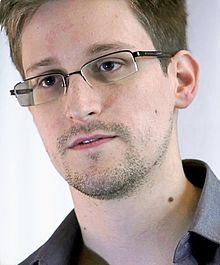
\includegraphics[scale=0.4] {./Illustrations/snowden.jpg} 
\end{center}
Le chiffrement fonctionne. Correctement mis en œuvre, les systèmes cryptographiques forts sont l'une des rares choses sur lesquelles vous pouvez compter.
}
\end{frame}


%----------------------------------------------------------------------------------------
\begin{frame}
\Huge{\centerline{Merci de votre attention.}}
\Huge{\centerline{Place aux questions. Débattons...}}

\end{frame}

%----------------------------------------------------------------------------------------
\begin{frame}
\frametitle{Et toi tu chiffres?}
\begin{center}
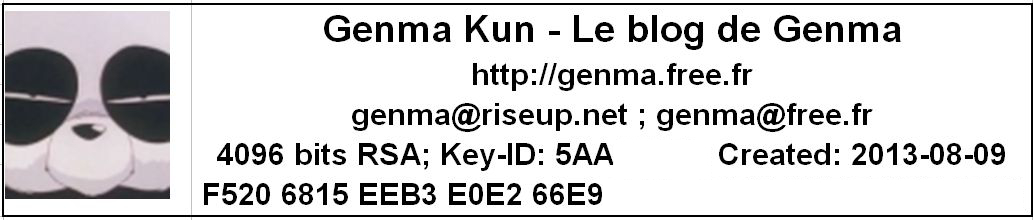
\includegraphics[scale=0.3] {./Illustrations/clef_papier.jpg} 
\\
 
\includegraphics[scale=0.3] {./Illustrations/https_everywhere_new_logo.jpg} 
 
\includegraphics[scale=0.5] {./Illustrations/seahorse.jpg} 
 
\includegraphics[scale=0.3] {./Illustrations/thunderbird.png} 
 
\includegraphics[scale=0.3] {./Illustrations/truecrypt.png} 
 
\includegraphics[scale=0.3] {./Illustrations/tor.png} 
\end{center}
\end{frame}


%----------------------------------------------------------------------------------------
\begin{frame}
\frametitle{L'audit de TrueCrypt}
\begin{center}
 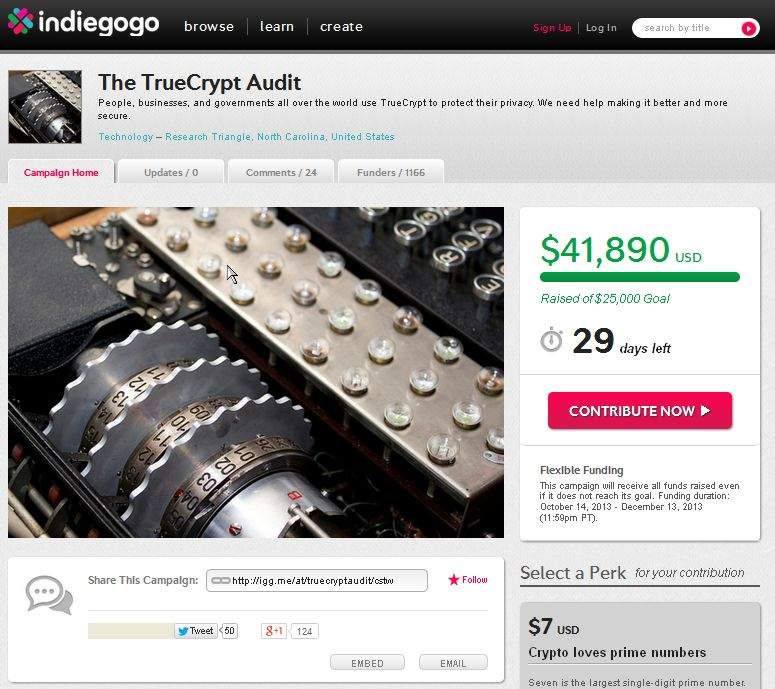
\includegraphics[scale=0.45] {./Illustrations/truecryptaudit.jpg} 
\end{center}
\end{frame}

%----------------------------------------------------------------------------------------
\begin{frame}
\frametitle{Le crypto-anarchisme}
Tout le monde chiffre et ce qui est vraiment important est chiffré et noyé dans la masse.
\\~\\
On crée du bruit ce qui empêche la surveillance de masse (Affaire PRISM...)
\\~\\
Attention, à l'heure actuel, le chiffrement étant peu répandu, toute personne qui chiffre ses e-mails pourra être considérée comme suspecte.
\end{frame}

%----------------------------------------------------------------------------------------
\begin{frame}

\frametitle{Chiffrer son disque dur}
\begin{block}{Logiciels intégrés aux systèmes d'exploitations}
\begin{itemize}
\item Windows 7/8 : Bitlocker
\item MacOS : FileVault
\item GNU/Linux : Encfs
\end{itemize}
\end{block}

\begin{block}{Indépendament du système d'exploitation}
$\Rightarrow$ Le logiciel TrueCrypt. Pour une clef USB/un disque dur externe.
\end{block}
\end{frame}

\begin{frame}
\frametitle{Annexes}
\begin{block}{La fonction de hashage}
\justifying{
\begin{itemize}
\item Un hash est une fonction à sens unique permettant le calcul d'une empreinte.
\item C'est une somme de contrôle qui permet de vérifier l'intégrité d'un fichier.
\item C'est une façon de cacher quelque chose.
\end{itemize}
}
La phrase  \og Nous venons en paix \fg devient  \\9d6bd655e000f83685d64affde380a3d94a62d47d42d80a0be11a4bb4c6ee324
\end{block}
\end{frame}

\end{document}
